% Select Arial font for the whole document
\usepackage{helvet}
\renewcommand{\familydefault}{\sfdefault}


\usepackage[a4paper, includehead,
textwidth=16cm, textheight=23cm,
headheight=2.7cm,
%showframe,
]{geometry}


\usepackage{fancyhdr}

% AD and RD entries
\usepackage{enumerate}
\usepackage[shortlabels]{enumitem}

\newenvironment{ADlist}
               {\begin{enumerate}[start=1,label={AD\arabic*}]}  % \bfseries
               {\end{enumerate}}               
\newenvironment{RDlist}
               {\begin{enumerate}[start=1,label={RD\arabic*}]}  % \bfseries
               {\end{enumerate}}
\newcommand{\ARDitem}[2]{\item \label{#1} {#2}}
\newcommand{\citedoc}[1]{[\ref{#1}]}


% List of requirements
\usepackage{tocloft}
\newcommand{\listreqname}{List of Requirements:}
\newlistof{req}{toreq}{\listreqname}
\newcommand{\req}[2]{%
\refstepcounter{req}
\par\vspace{0.2cm}\noindent\textbf{\esoreqprefix{}\thereq:} #2 \label{#1}\vspace{0.2cm}
\addcontentsline{toreq}{req}
{\protect \textbf{\esoreqprefix{}\numberline{\thereq}}#2}\par}
\newcommand{\citereq}[1]{\textbf{\esoreqprefix{}\ref{#1}}}


% List of questions
\newcommand{\listquestionname}{List of Questions:}
\newlistof{question}{toquestion}{\listquestionname}
\newcommand{\question}[2]{%
\refstepcounter{question}
\par\vspace{0.2cm}\noindent\textbf{Q\thequestion:} #2 \label{#1}\vspace{0.2cm}
\addcontentsline{toquestion}{question}
{\protect \textbf{Q\numberline{\thequestion}}#2}\par}
\newcommand{\citequestion}[1]{\textbf{Q\ref{#1}}}


% Title page
\newcommand{\esotitlepage}[1]{
\thispagestyle{empty}
\begingroup
%\setlength{\tabcolsep}{10pt}       % Default value: 6pt
\renewcommand{\arraystretch}{1.5}   % Default value: 1
\begin{center}
  \begin{tabular}{|p{0.3\textwidth}|p{0.7\textwidth}|}
    \hline
        {\bf \small Document title:}          & {\bf \esodoctitle{}}         \\[0.8cm] \hline
        {\bf \small Document number:}         &      \esodocnumber{}         \\[0.8cm] \hline
        {\bf \small Document verision:}       &      \esodocversion{}        \\[0.8cm] \hline
        {\bf \small Document type:}           &      \esodoctype{}           \\[0.8cm] \hline
        {\bf \small Document status:}         &      \esodocstatus{}         \\[0.8cm] \hline
        {\bf \small Releasing organization:}  &      \esodocorganization{}   \\[0.8cm] \hline
        {\bf \small Released on:}             &      \esodocreleasedate      \\[0.8cm] \hline
        {\bf \small Document classification:} &      \esodocclassification{} \\[0.8cm] \hline
  \end{tabular}
\end{center}

\vspace{3cm}

#1

\endgroup

\newpage

}



% Running header
\newcommand{\esoheader}{
\pagestyle{fancy}
\fancyhead{} % clear all header fields
\fancyfoot{} % clear all footer fields
\renewcommand{\headruleskip}{1.2mm}
\fancyhead[L]{
  \begin{tabular}{m{0.12\headwidth}p{0.34\headwidth}}
    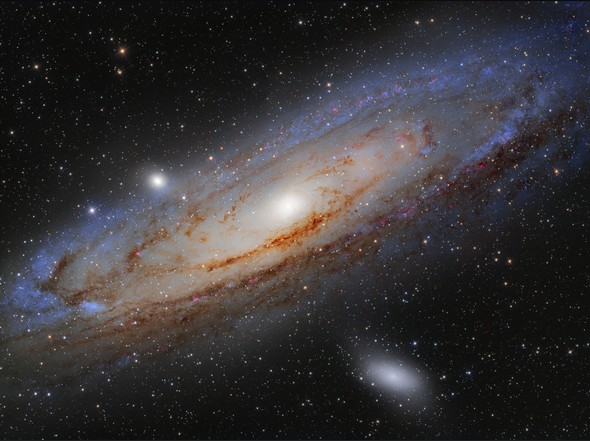
\includegraphics[width=2.2cm]{media/header_logo.jpg}  &  {\small \esodoctitle{}}\\
  \end{tabular}
}
\fancyhead[R]{
    \footnotesize
    \begin{tabular}{|p{0.2\headwidth}|p{0.21\headwidth}|}
      \hline
        {Document number:}         &      \esodocnumber{}     \\\hline
        {Document verision:}       &      \esodocversion{}    \\\hline
        {Document status:}         &      \esodocstatus{}     \\\hline
        {Released on:}             &      \esodocreleasedate  \\\hline
        {Page:}                    &      \thepage{} of \pageref{LastPage} \\\hline
    \end{tabular}
}
}
